\documentclass[12pt]{article}
\usepackage[hidelinks]{hyperref}
\usepackage{graphicx, amsmath, listings, amssymb, commath, enumitem, listingsutf8, float}
\usepackage[utf8]{inputenc}
\usepackage[slovene]{babel}
\setlist[enumerate]{font=\large\bfseries}
\setlist[itemize]{font=\normalsize\bfseries}
\lstdefinestyle{mystyle}{
	showtabs=false, 
	tabsize=2
}

\lstdefinestyle{mystyle}{
	showtabs=false, 
	tabsize=2
}
\lstset{style=mystyle}
\usepackage[utf8]{inputenc}

\title{\small{2. projekt pri predmetu MATEMATIČNO MODELIRANJE} \\ \hfill \\ \hfill \\ \huge{\textbf{Presek dveh implicitno danih ploskev}}}
\author{Aljaž Verlič, Lina Lumborovska, Blažka Blatnik, Luka Tavčer \\
	Mentor: Damir Franetič}
\date{5. junij, 2017}
\begin{document}
	
	
	\maketitle
	\newpage
	\textbf{\large{Vsebina}} 
	\begin{enumerate}
		\item Predstavitev problema
		\item Opis modela in uporabljenih metod
		\item Potrebni pogoj in Jacobijeva matrika
		\item Adaptivni korak
		\item Implementacija, testiranje in primeri
		\item Analiza za povprečno število korakov Newtonove metode
		\item Koda
		\item Delitev dela v skupini
		\item Reference
	\end{enumerate} 
	\newpage
	
	\section{Predstavitev problema}
	V $\mathbb{R}^3$ imamo podani dve poljubni implicitno dani ploskvi, opisani z enačbama $f_{1}(x)$ = $C_{1}$ in $f_{2}(x)$ = $C_{2}$. Presek teh dveh ploskev je množica rešitev nelinearnega sistema enačb:
	\begin{center}
		$f_{1}(x)$ = $C_{1}$,\\$f_{2}(x)$ = $C_{2}$.
	\end{center}
	Naša naloga je poiskati krivuljo $K$ (oziroma točke na njej), ki predstavlja presek teh dveh ploskev. \\
	
	\section{Opis modela in uporabljenih metod}
	Sistem lahko gledamo tudi, kot enačbe nivojnic funkcij  $f_{1}$ in $f_{2}$, krivulja K pa je presek teh nivojnic. Gradienta funkcij sta tako v vsaki točki krivulje preseka pravokotna nanjo. To opišemo:
	\begin{center}
		$F(x) = \dfrac{(grad f_{1}(x))\times(grad f_{2}(x))}{\|grad f_{1}(x))\times(grad f_{2}(x))\|}$
	\end{center}
	in označimo z $x = x(t)$ naravno parametrizacijo krivulje K. Ta x je rešitev avtonomnega sistema diferencialnih enačb:
	\begin{center}
		$\dot{x} = F(x)$
	\end{center}
	
	\subsection{Reševanje sistema diferencialnih enačb}
	Za reševanje sistema diferencialnih enačb lahko uporabimo katero izmed dveh znanih metod za numerično reševanje diferencialnih enačb.
	\subsubsection{Eulerjeva metoda}
	Eulerjeva metoda je numerična metoda za reševanje diferencialnih enačb, z podanim začetnim približkom. Prednost metode je, da je preprosta in najbolj logična. Na vsakem koraku naslednjo točko $(x_{i+1},y_{i+1})$ dobimo tako, da se za korak $h$ premaknemo vzdolž tangente na rešitev $(x_{i},y_{i})$. Geometrijsko lahko delovanje metode predstavimo s spodnjo sliko.
	
	\begin{figure}[H]
		\centering
		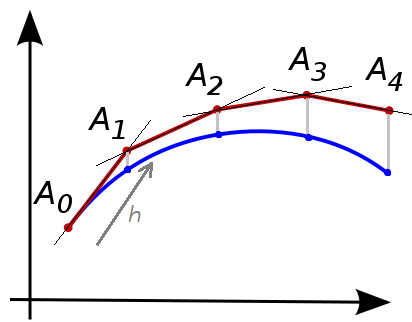
\includegraphics[width=0.5\textwidth]{Euler_method_geom}
		\caption{Geometrijski prikaz delovanja Eulerjeve metode.}
		\label{slika:Euler_method_geom}
	\end{figure}
	
	Slabost opisanega postopka je napaka, ki se skozi iteracije izvajanja metode povečuje (napaka na vsakem koraku metode je reda $O(h^2)$, kumulativna napaka pa z vsako iteracijo narašča). Tako je napaka večja, tem večji je korak. V iskanju rešitve našega problema to predstavlja težavo, zato moramo vsak izračunan približek vedno popraviti tako, da spet leži na krivulji preseka. 
	Na preprostem primeru iskanja presečišč valja in sfere lahko opazimo delovanje Eulerjeve metode in problem kumulativne napake (valja na sliki zaradi večje preglednosti ni)
	
	\begin{figure}[H]
		\centering
		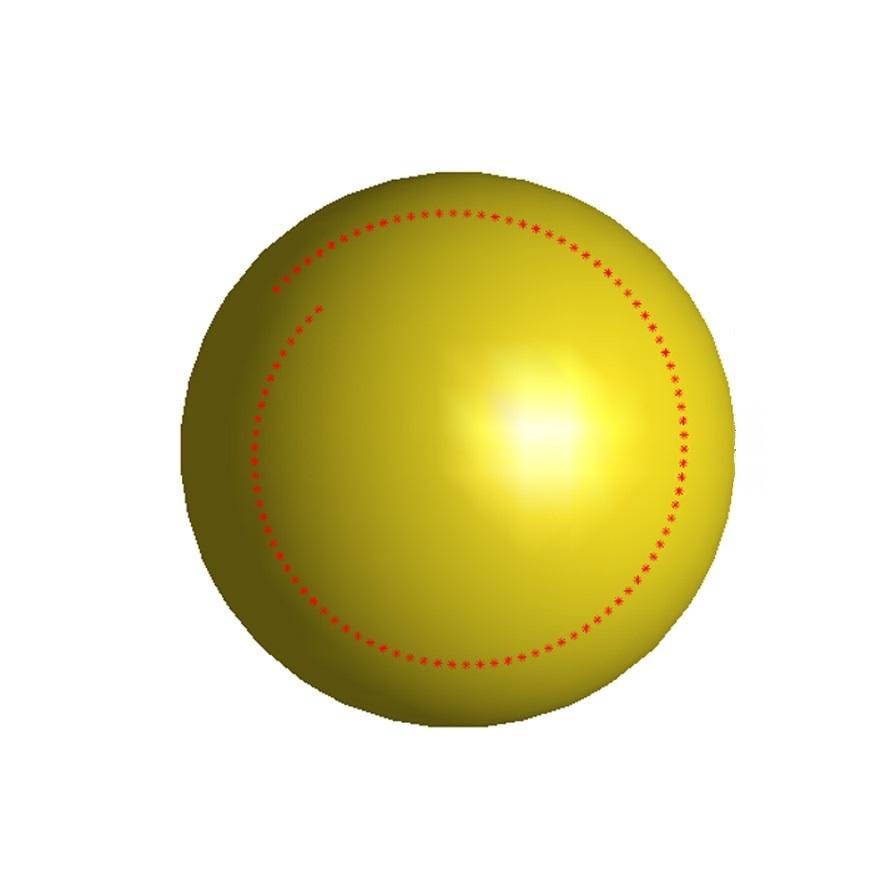
\includegraphics[scale=0.30]{eul1}
		\caption{Eulerjeva metoda z manjšim korakom}
		\label{slika:eul1}
	\end{figure}
	\begin{figure}[H]
		\centering
		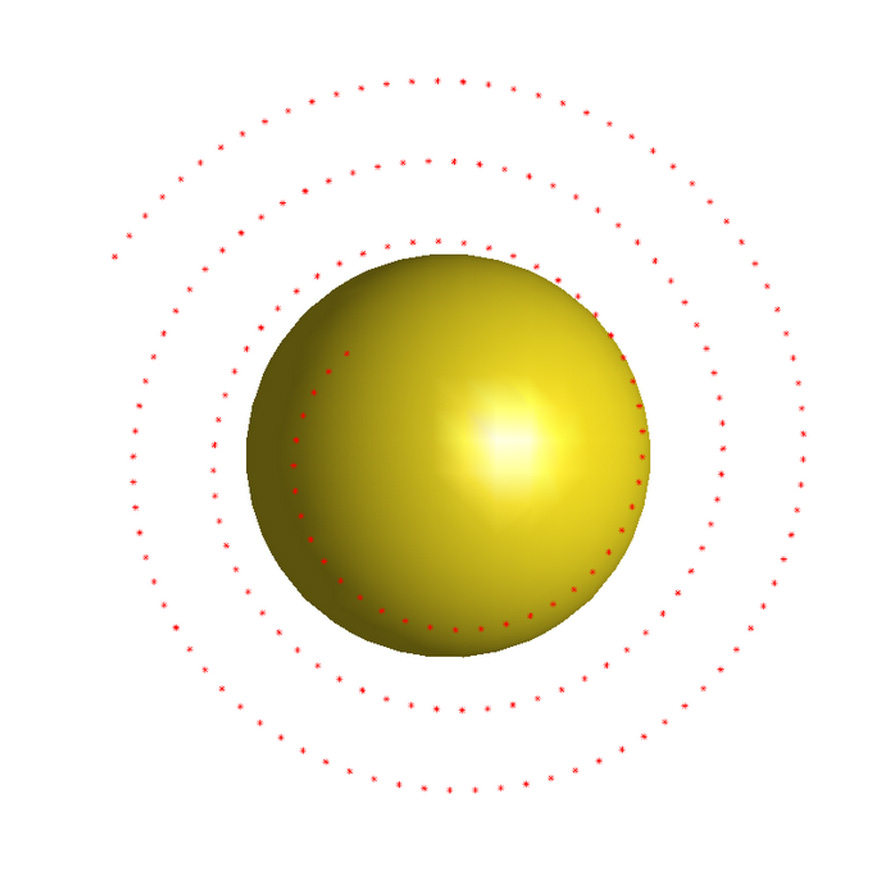
\includegraphics[scale=0.30]{eul2}
		\caption{Eulerjeva metoda z večjem korakom}
		\label{slika:eul2}
	\end{figure}
	
	
	\subsubsection{Metoda Runge-Kutta 4}
	Precej bolj natančna, a manj intuitivna metoda za reševanje diferencialnih enačb, je metoda Runge-Kutta 4. Tudi tu potrebujemo nek začetni približek, metoda pa potem z večjo natančnostjo računa nadaljne premike. Kumulativna napaka je konstantna in se za razliko od Eulerjeve z iteracijami ne povečuje.
	
	\subsubsection{Newtonova metoda za popravljanje približkov}
	Pri uporabi Eulerjeve metode je potrebno sprotno popravljanje približkov, saj se drugače napake seštevajo do te mere, da ne dobimo željene rešitve.\\
	Dobljeni približek y, želimo popraviti na nek x, ki bo ležal na preseku. Če zapišemo $F(y) \cdot x = F(y)\cdot y $, nam to predstavlja enačbo ravnine, ki je zelo blizu normalni ravnini na krivuljo K. Z Newtonovo metodo z začetnim približkom y rešimo sistem enačb:
	\begin{center}
		$f_{1}(x)$ = $C_{1}$\\$f_{2}(x)$ = $C_{2}$\\ $F(y) \cdot x = F(y)\cdot y $
	\end{center}
	Rešitev sistema je točka, ki leži na presečišču obeh ploskev. V primeru uporabe RK4 je Newtonova metoda bolj potrebna predvsem za postavitev začetnega približka na presečišče, saj je metoda RK4 že sama po sebi precej natančna. Učinkovitost metode je razvidna iz primerov:
	
	\begin{figure}[H]
		\centering
		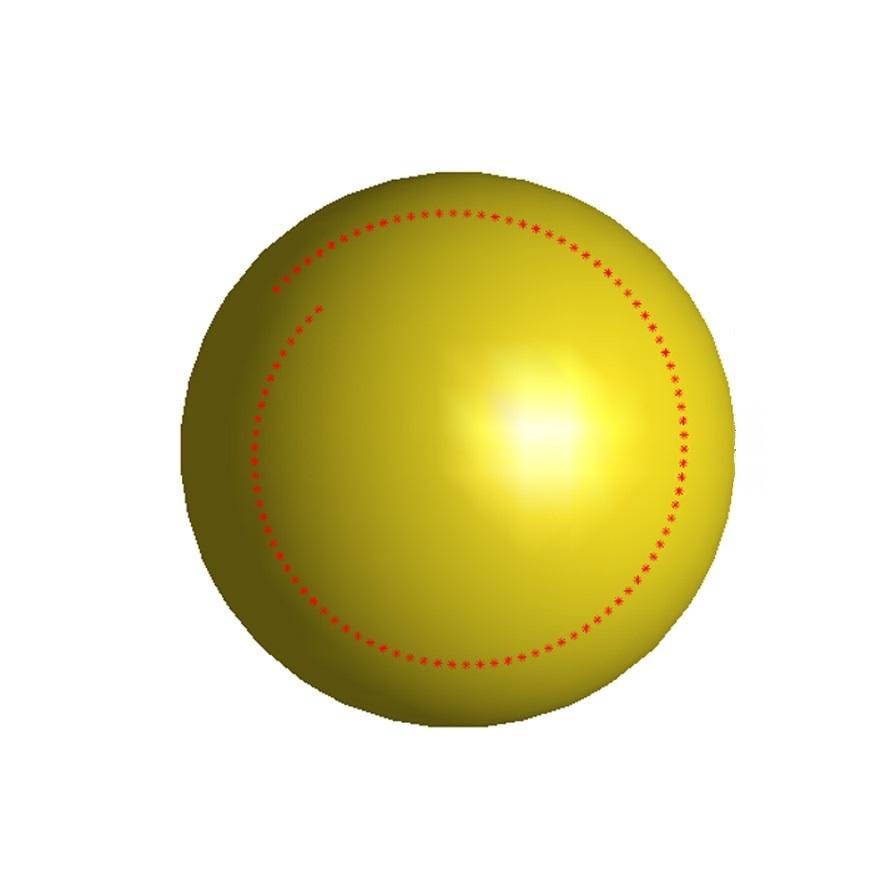
\includegraphics[scale=0.3]{eul1}
		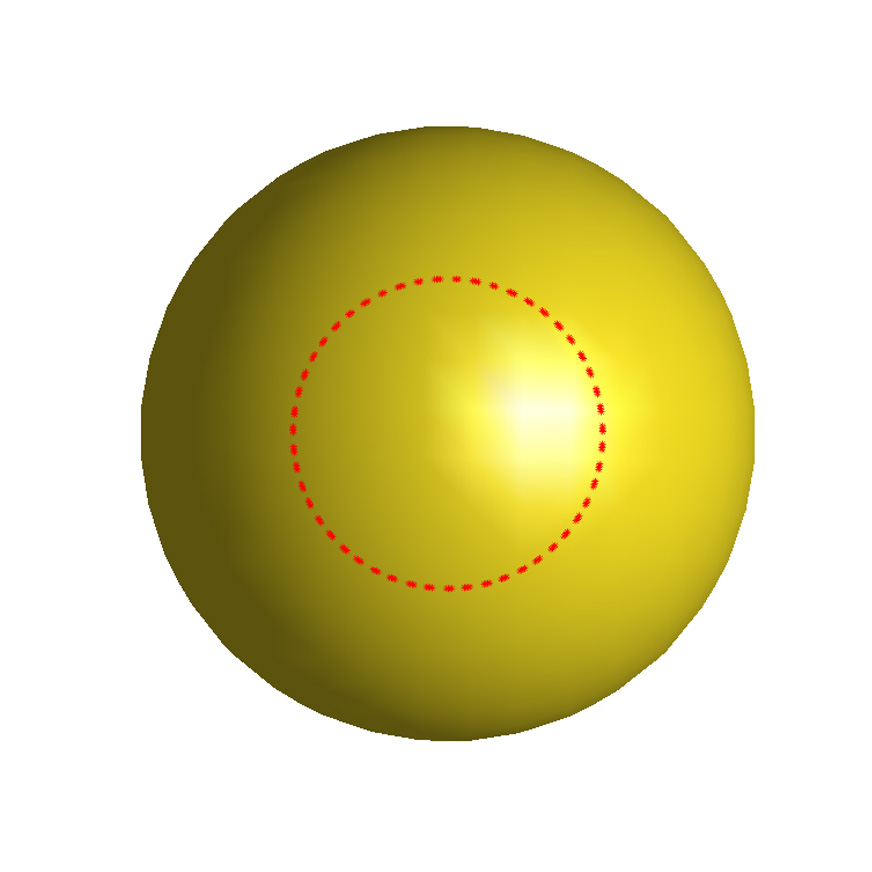
\includegraphics[scale=0.3]{eul3_newt}
		\caption{Osnovna Eulerjeva metoda (levo) in popravljena Eulerjeva metoda (desno).}
		\label{slika:eul1,eul3_newt}
	\end{figure}
	\begin{figure}[H]
		\centering
		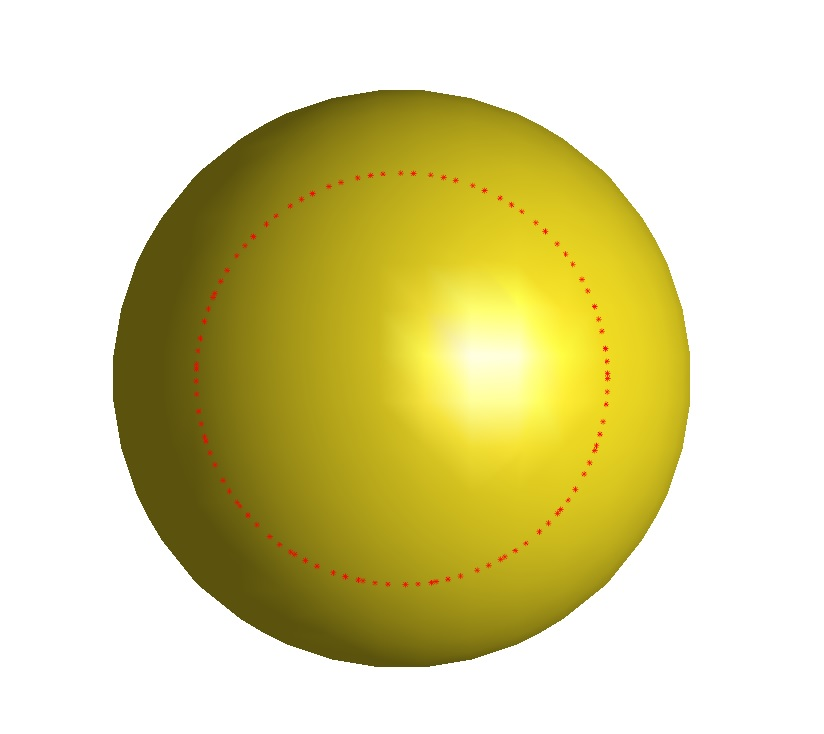
\includegraphics[scale=0.30]{rk4}
		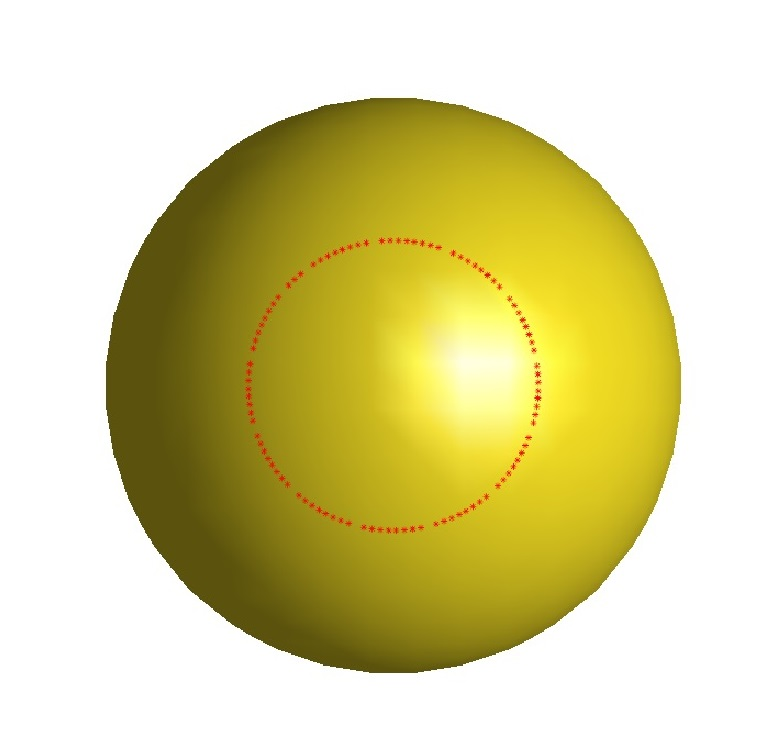
\includegraphics[scale=0.30]{rk4_newt}
		\caption{Osnovna metoda RK4 (levo) in popravljena metoda RK4 (desno).}
		\label{slika:rk4,rk4_newt}
	\end{figure}
	
	\newpage	
	\section{Potreben pogoj in Jacobijeva matrika}
	Potreben pogoj za delovanje metod je, da sta funkciji $f_{1}$ in $f_{2}$ parcialno odvedljivi in da ima Jacobijeva matrika parcialnih odvodov poln rang 2. Za uspešno delovanje Newtonove metode moramo poiskati Jacobijevo matriko leve strani sistema nelinearnih enačb:
	
	\begin{center}
		JG = $\begin{bmatrix}
		grad(f_{1}) \\
		grad(f_{2}) \\
		\hspace{1mm}grad(\vec{v} \cdot \vec{x}) \\
		\end{bmatrix}$
		oziroma
		JG = $\begin{bmatrix}
		grad(f_{1}) \\
		grad(f_{2}) \\
		\hspace{1mm}grad(\vec{v}\hspace{0.5mm}^\intercal) \\
		\end{bmatrix}$
	\end{center}
	Newtnova metoda rešuje sistem:
	\begin{center}
		$\vec{F}(\vec{x}) = \vec{0}$,
	\end{center}
	zato je potrebno poiskati tudi matriko $\vec{F}(\vec{x})$, ki je enaka:
	\begin{center}
		$\vec{F}(\vec{x})$ = $\begin{bmatrix}
		f_{1}(\vec{v}) - C_{1} \\
		f_{2}(\vec{v}) - C_{2} \\
		\hspace{1mm}\vec{v} \cdot \vec{x} - \vec{v} \cdot \vec{y}) \\
		\end{bmatrix}$
	\end{center}
	
	\section{Adaptivni korak}
	Adaptivni korak omogoča natančnejšo rešitev problema, saj dinamično prilagaja dolžino koraka. Tako lahko na bolj preprostih predelih preseka uporabljamo večji korak in je metoda hitrejša, na kompleksnejših delih preseka, kjer je potrebna večja natančnost, pa se premikamo z manjšim korakom. Program poveča oziroma zmanjša korak glede na število korakov, ki jih izvede Newtonova metoda za eno točko. Empirično smo določili, da je velikost koraka $h$ na intervalu $h\in[10^{-7},100]$ in da se korak povečuje oziroma zmanjšuje s faktorjem 2. Korak se ne spremeni, če je število korakov enako 2 ali 3.
	
	\begin{figure}[H]
		\centering
		\begin{minipage}{.5\textwidth}
			\centering
			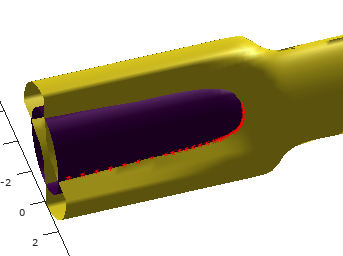
\includegraphics[scale=0.50]{slikaAda}
			\caption{Adaptivni korak}
			\label{slika:slikaAda}
		\end{minipage}%
		\begin{minipage}{.5\textwidth}
			\centering
			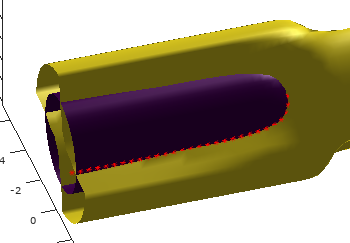
\includegraphics[scale=0.50]{slikaAda2}
			\caption{Brez adaptivnega koraka}
			\label{slika:slikaAda2}
		\end{minipage}
	\end{figure}		
	
	\section{Implementacija, testiranje in primeri}
	Delovanje našega programa lahko preverimo s programom, ki smo ga napisali v Octave-u. Kot vhodne parametre mu podamo obe implicitno podani funkciji $f_{1}$, $f_{2}$, $C1$, $C2$, $grad(f_{1})$, $grad(f_{2})$. Določimo tudi začetni približek $x_{0}$, začetno dolžino koraka in pa parameter, ki določa metodo delovanja (Euler/Runge-Kutta).\\
	Program poženemo na različnih primerih in štejemo povprečno dolžino koraka ter število porabljenih korakov:\\\\
	
	\begin{minipage}{\textwidth}
		\textbf{\large{Primer 1:}}
		\begin{itemize} 
			\item $f_{1}(x,y,z)$ = $x^2 + y^2 + z^2$ = 4
			\item $f_{2}(x,y,z)$ = $3x + 2y + z$ = 1	
		\end{itemize}
		\begin{figure}[H]
			\centering
			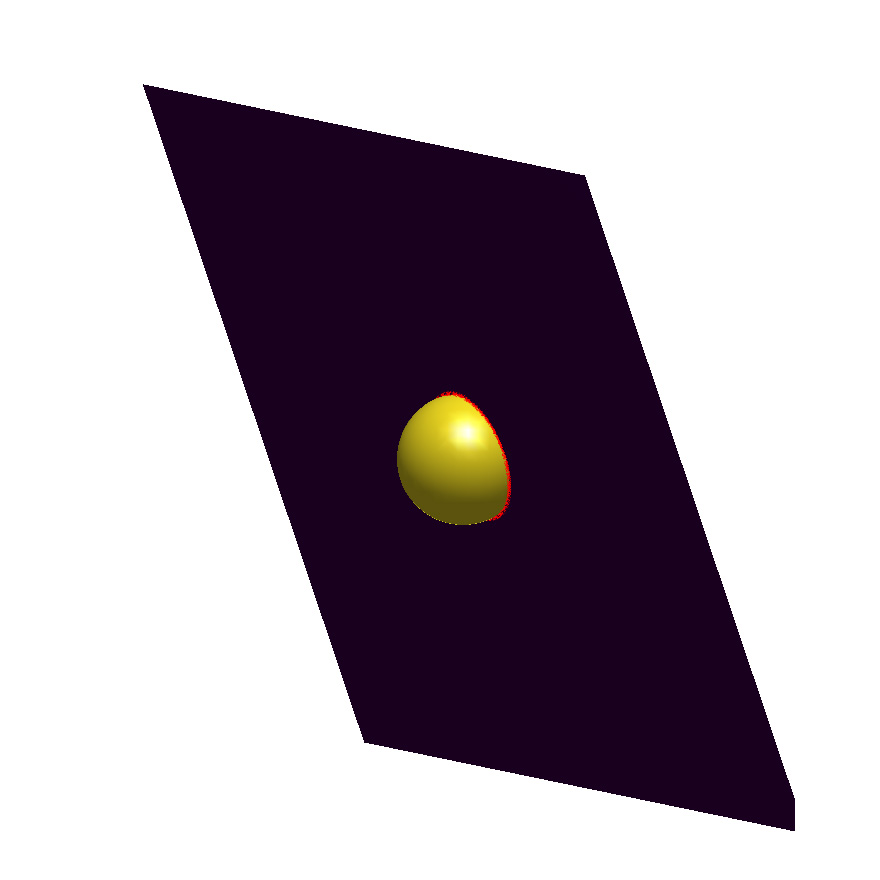
\includegraphics[scale=0.3]{primer1_1}
			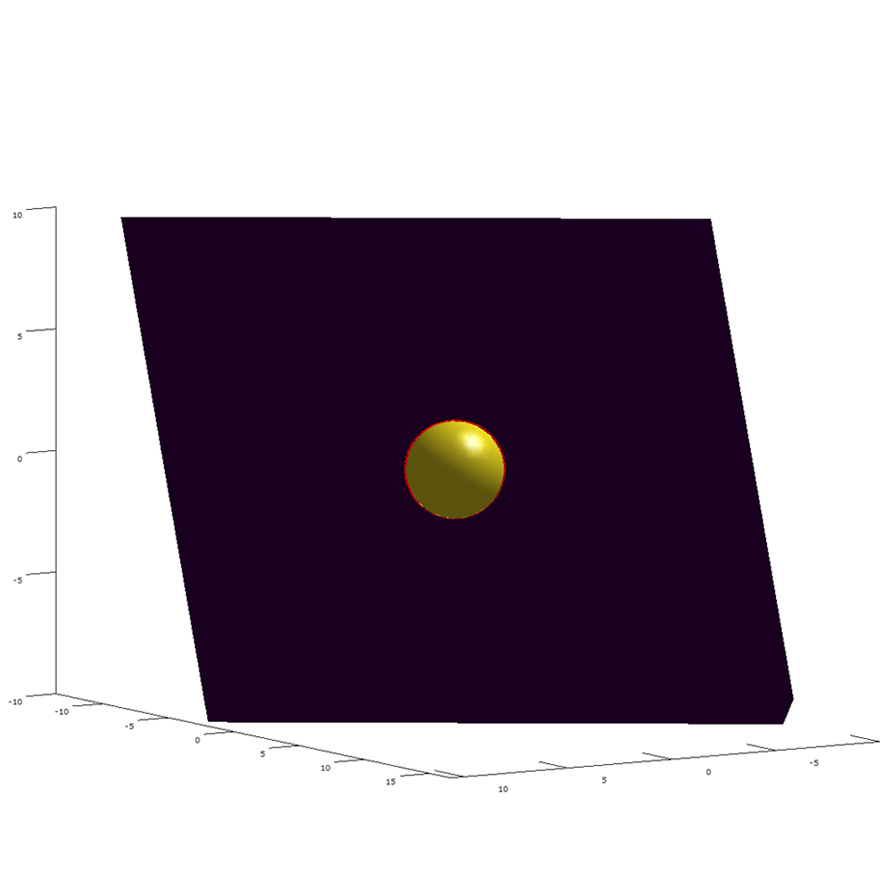
\includegraphics[scale=0.3]{primer1_2}
		\end{figure}
	\end{minipage}
	
	\begin{minipage}{\textwidth}
		\textbf{\large{Primer 2:}}
		\begin{itemize}  
			\item $f_{1}(x,y,z)$ = $x^2 + y^2 + z^2$ = 4
			\item $f_{2}(x,y,z)$ = $x^2 + y^2$ = 1
		\end{itemize}
		\begin{figure}[H]
			\centering
			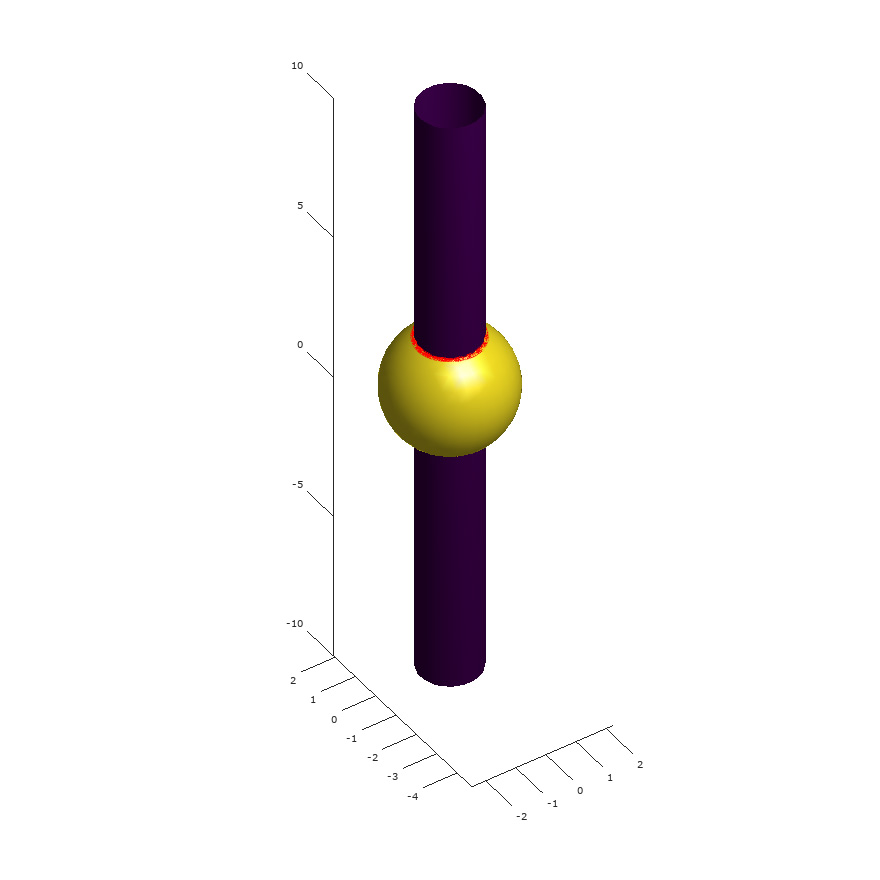
\includegraphics[scale=0.3]{primer2_1}
			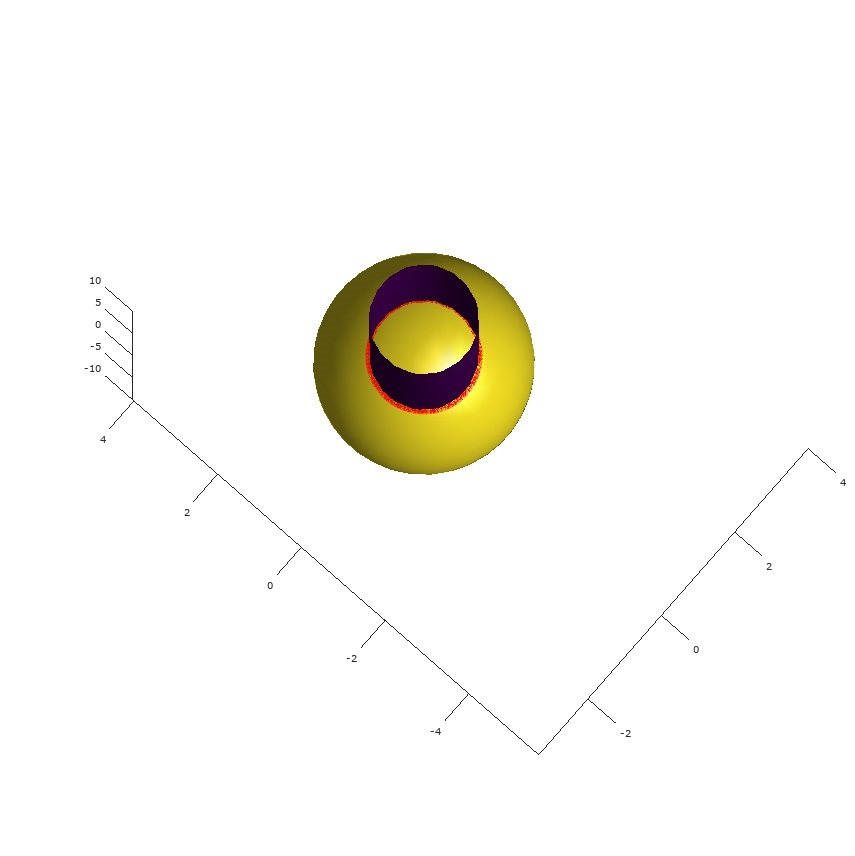
\includegraphics[scale=0.3]{primer2_2}
		\end{figure}
	\end{minipage}
	
	\begin{minipage}{\textwidth}
		\textbf{\large{Primer 3:}}
		\begin{itemize}  
			\item $f_{1}(x,y,z)$ = $x^2 + y^2 + z^2$ = 4
			\item $f_{2}(x,y,z)$ = $y^4 + log(x^2 + 1)z^2 - 4$ = 1
		\end{itemize}
		\begin{figure}[H]
			\centering
			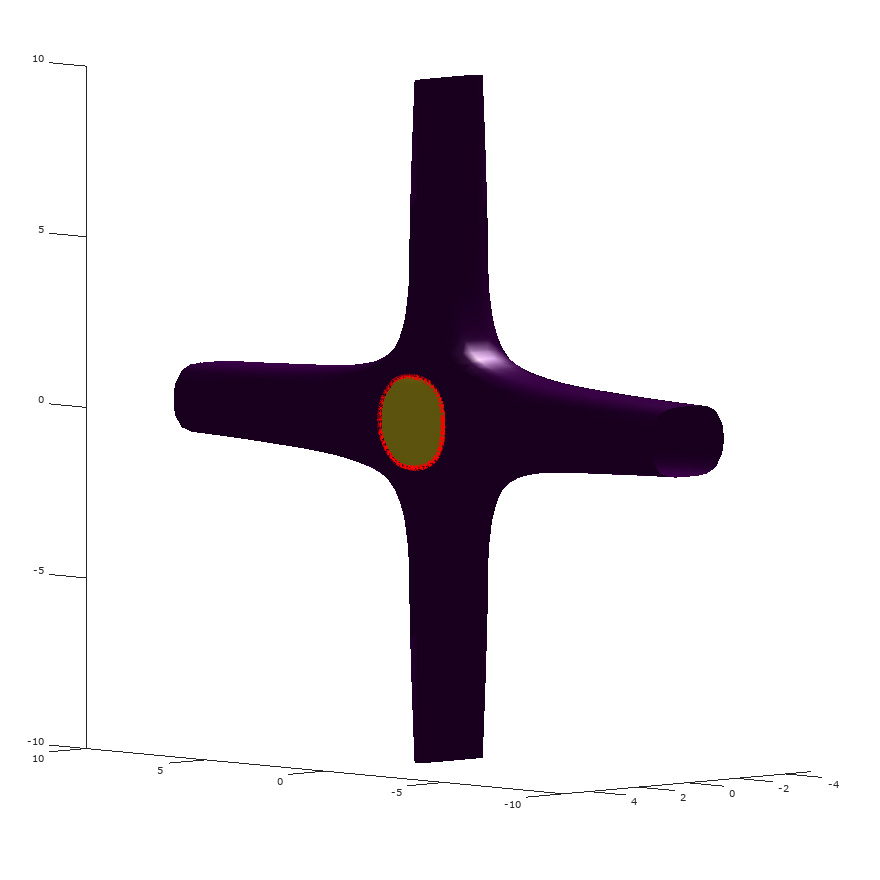
\includegraphics[scale=0.3]{primer3_1}
			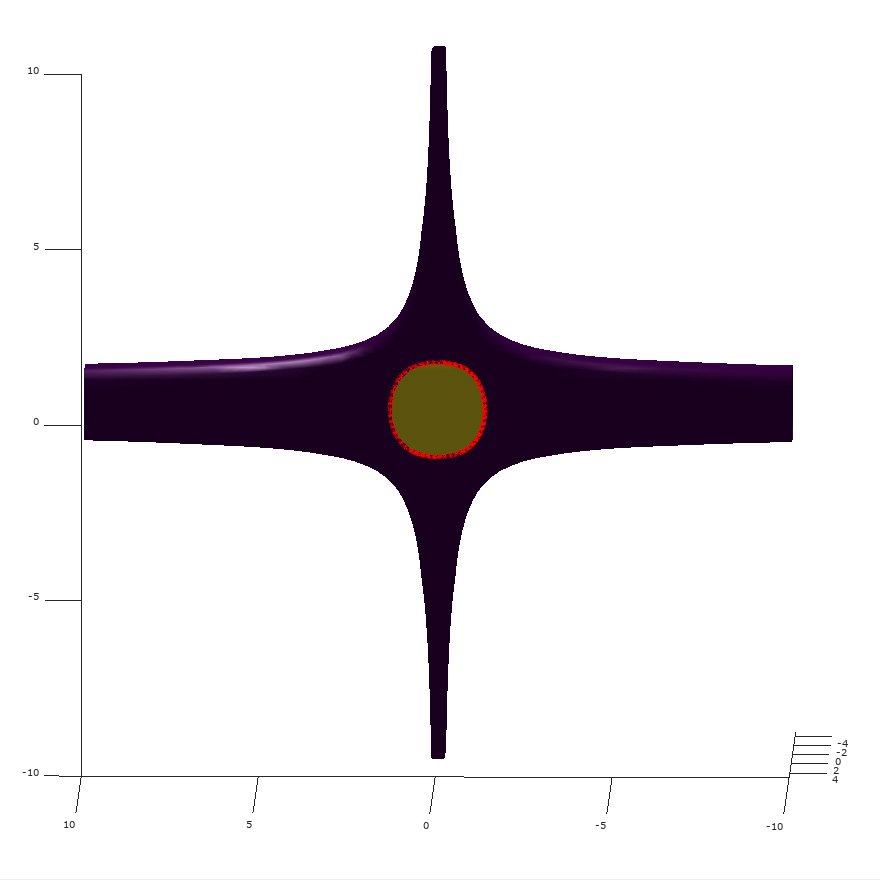
\includegraphics[scale=0.3]{primer3_2}
		\end{figure}
	\end{minipage}
	
	\begin{minipage}{\textwidth}
		\textbf{\large{Primer 4:}}
		\begin{itemize}  
			\item $f_{1}(x,y,z)$ = $x^2 + cos(y)z^2 - 12$ = 4
			\item $f_{2}(x,y,z)$ = $y^4 + log(x^2 + 1)z^2 - 4$ = 1
		\end{itemize}
		\begin{figure}[H]
			\centering
			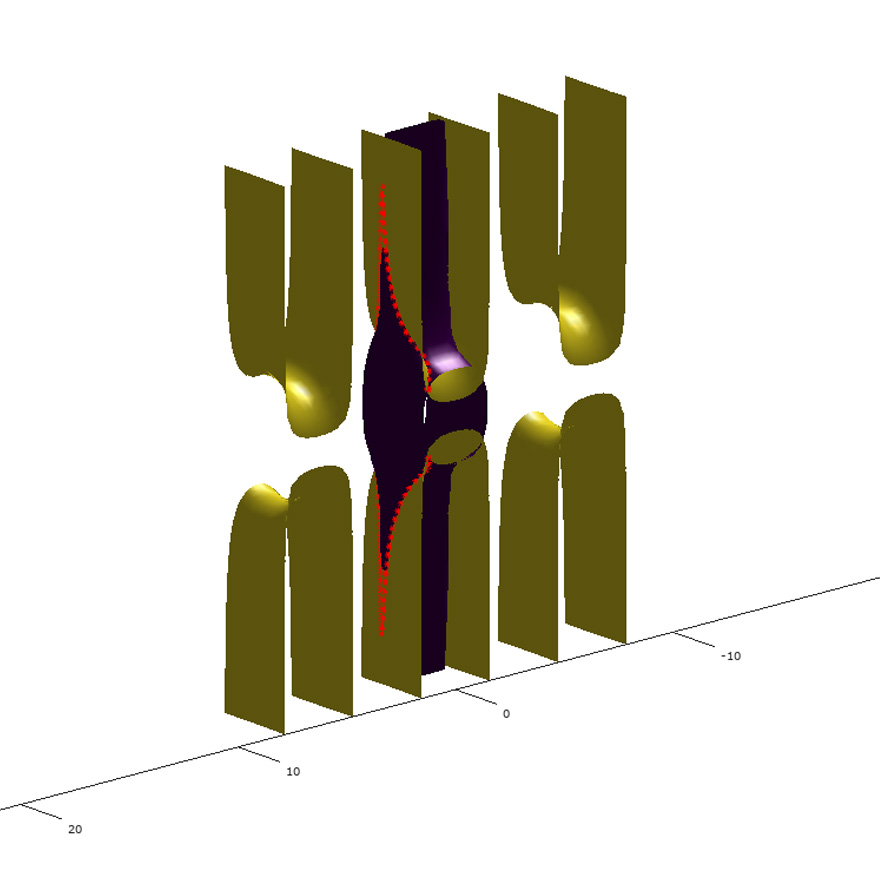
\includegraphics[scale=0.32]{primer4_1}
			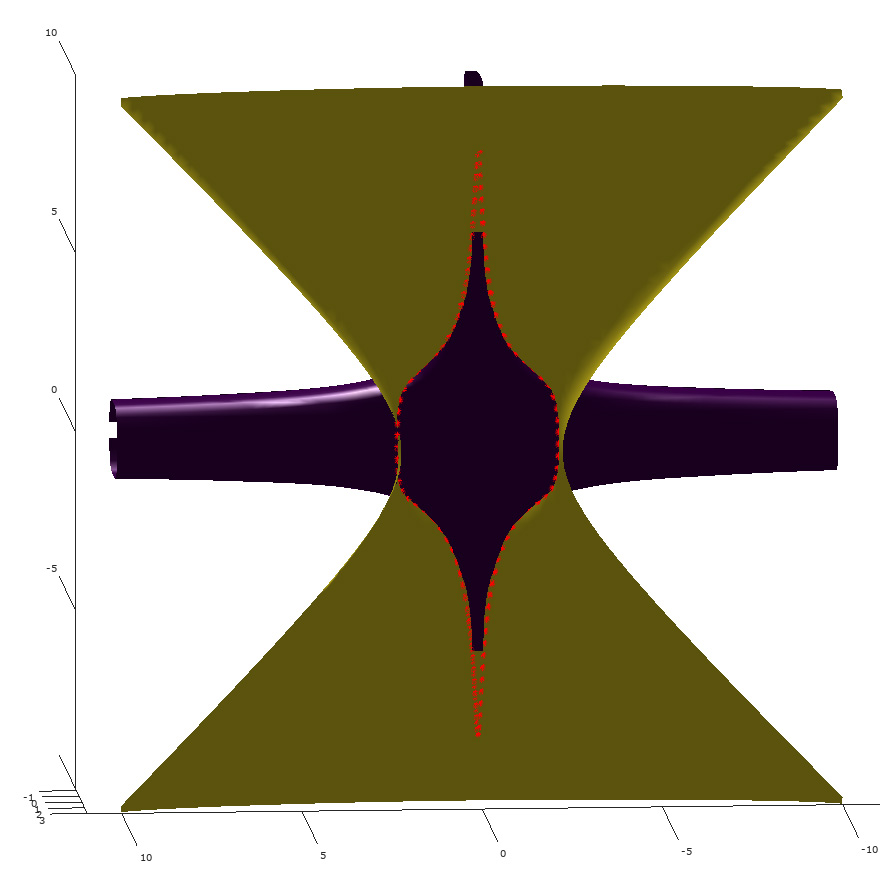
\includegraphics[scale=0.32]{primer4_2}
			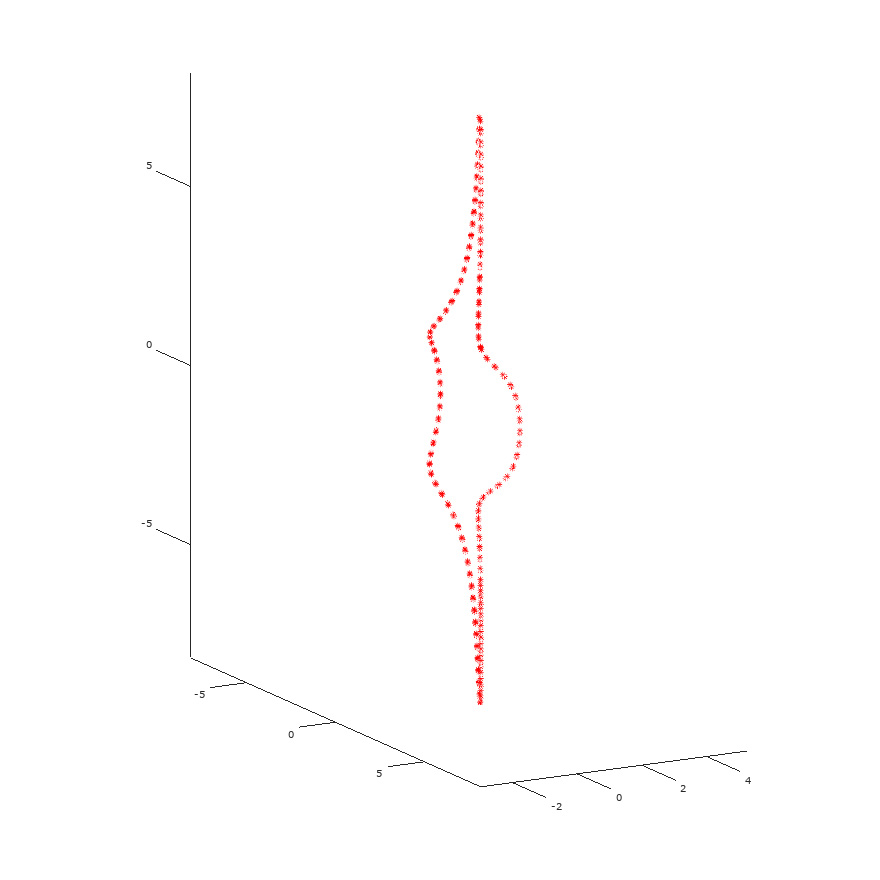
\includegraphics[scale=0.32]{primer4_4}
			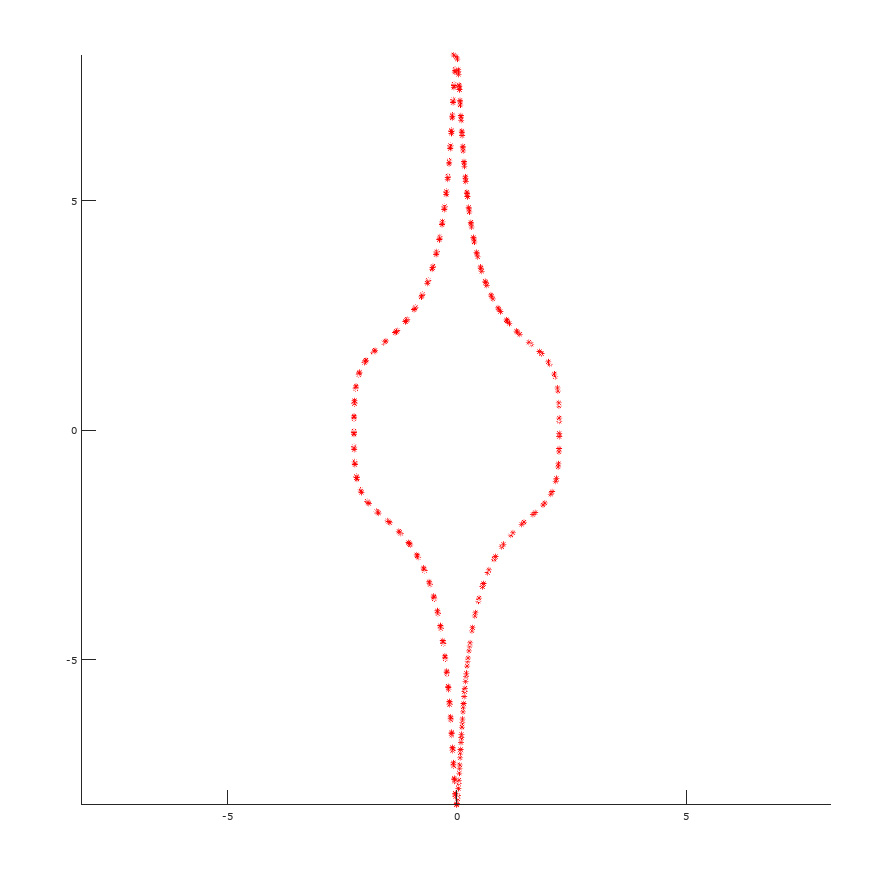
\includegraphics[scale=0.32]{primer4_3}
		\end{figure}
	\end{minipage}
	
	\begin{minipage}{\textwidth}
		\textbf{\large{Primer 5:}}
		\begin{itemize}  
			\item $f_{1}(x,y,z)$ = $e^{(-x^{2}+1)}+y^{2}+z^{2}$ = 3
			\item $f_{2}(x,y,z)$ = $e^{(xyz)}+y^{2}+z^{2}$ = 10
		\end{itemize}
		\begin{figure}[H]
			\centering
			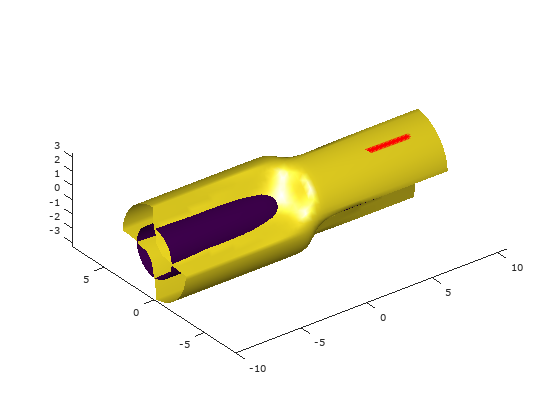
\includegraphics[scale=0.47]{primer5_1}
			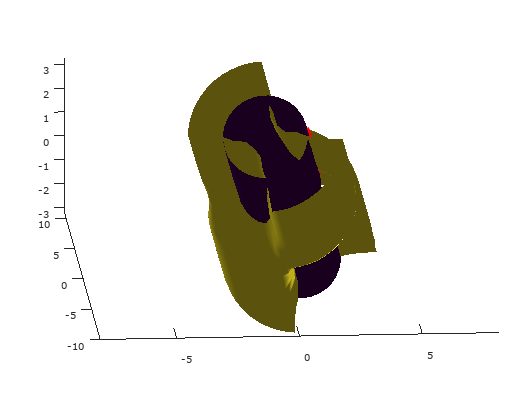
\includegraphics[scale=0.47]{primer5_2} 
			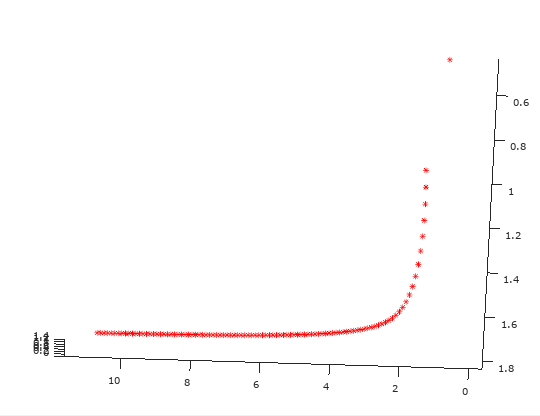
\includegraphics[scale=0.47]{primer5_3}
			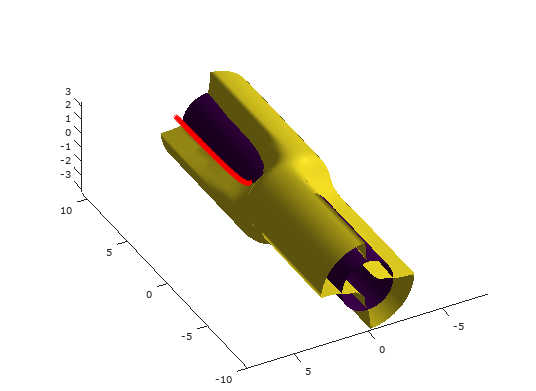
\includegraphics[scale=0.47]{primer5_4} 
		\end{figure}
	\end{minipage}
	
	\begin{minipage}{\textwidth}
		\textbf{\large{Primer 6:}}
		\begin{itemize}  
			\item $f_{1}(x,y,z)$ = $e^{(-x^{2}+1)}+y^{2}+z^{2}$ = 3
			\item $f_{2}(x,y,z)$ = $x^2 + y^2 + z^2$ = 4
		\end{itemize}
		\begin{figure}[H]
			\centering
			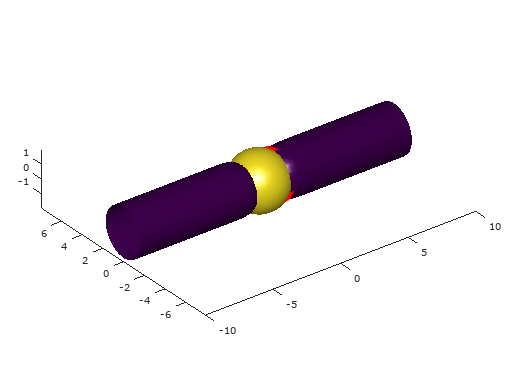
\includegraphics[scale=0.5]{primer6_1}
			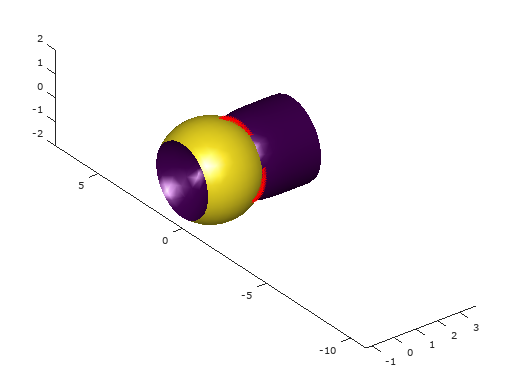
\includegraphics[scale=0.5]{primer6_2}
			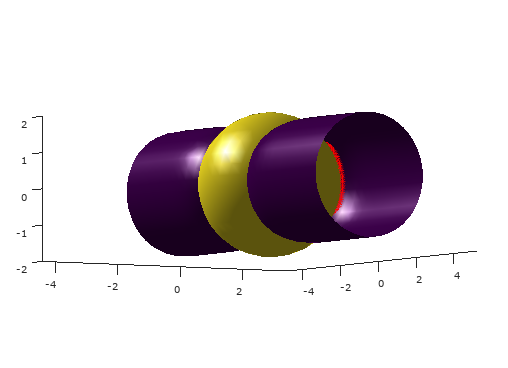
\includegraphics[scale=0.5]{primer6_3}
			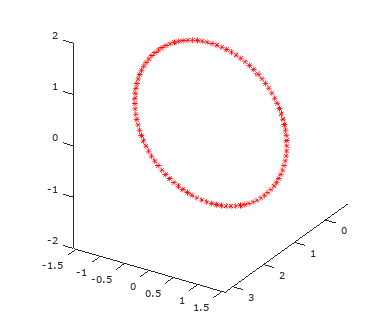
\includegraphics[scale=0.5]{primer6_4} 
		\end{figure}
	\end{minipage}
	
	\begin{minipage}{\textwidth}
		\textbf{\large{Primer 7:}}
		\begin{itemize}  
			\item $f_{1}(x,y,z)$ = $e^{(-x^{2}+1)}+y^{2}+z^{2}$ = 3
			\item $f_{2}(x,y,z)$ =  $x^2 + y^2$ = 1
		\end{itemize}
		\begin{figure}[H]
			\centering
			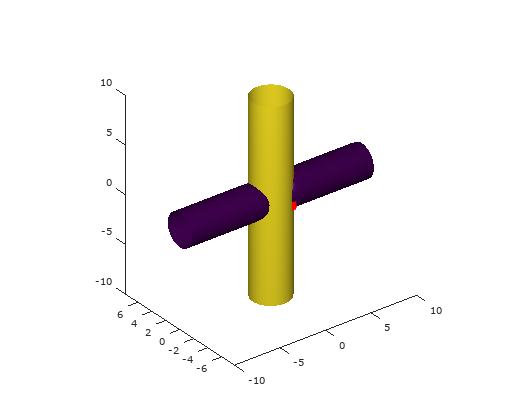
\includegraphics[scale=0.47]{primer7_1}
			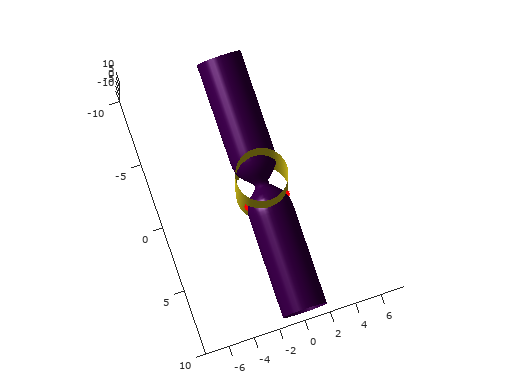
\includegraphics[scale=0.47]{primer7_2}
			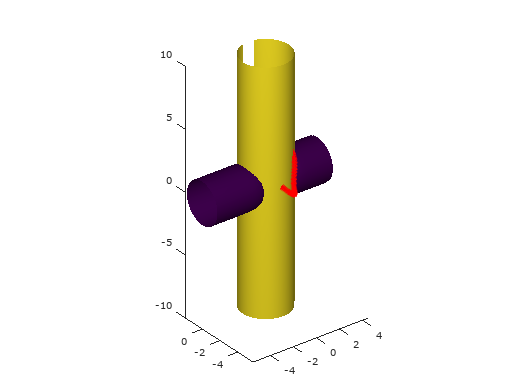
\includegraphics[scale=0.47]{primer7_3}
			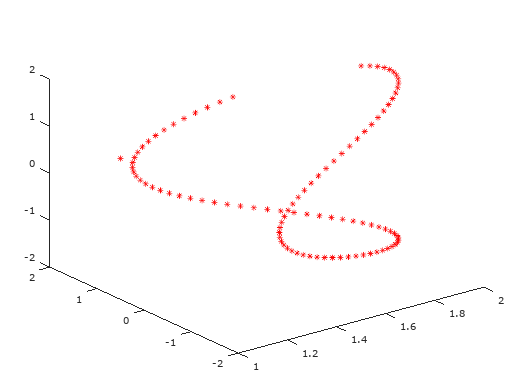
\includegraphics[scale=0.47]{primer7_4} 
		\end{figure}    
	\end{minipage}
	
	\begin{minipage}{\textwidth}
		\textbf{\large{Primer 8:}}
		\begin{itemize}  
			\item $f_{2}(x,y,z)$ = $e^{(xyz)}+y^{2}+z^{2}$ = 10
			\item $f_{2}(x,y,z)$ =  $x^2 + y^2$ = 1
		\end{itemize}
		\begin{figure}[H]
			\centering
			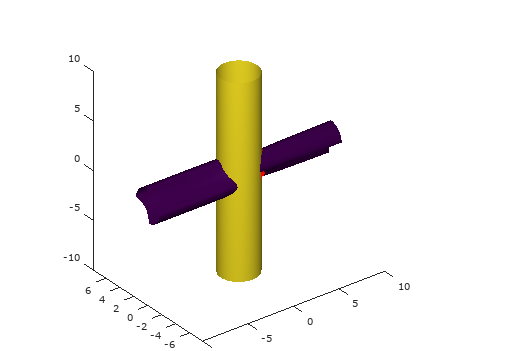
\includegraphics[scale=0.5]{primer8_1}
			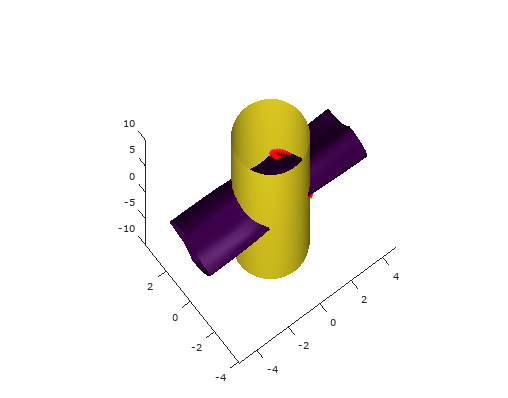
\includegraphics[scale=0.5]{primer8_2}
			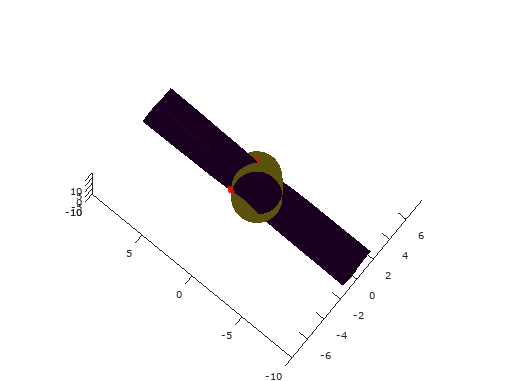
\includegraphics[scale=0.5]{primer8_3}
			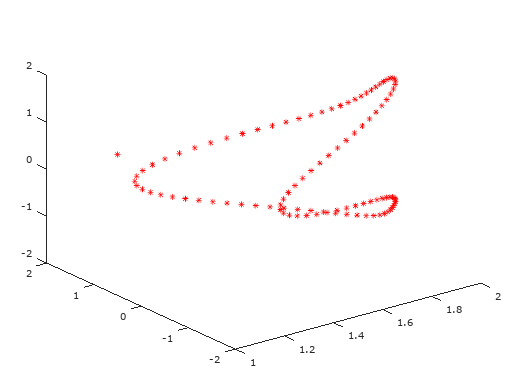
\includegraphics[scale=0.5]{primer8_4} 
		\end{figure} 
	\end{minipage}
	\newpage
	\section{Analiza povprečnega števila korakov Newtonove metode} 
	Na koncu smo za vseh 8 primerov naredili analizo, tako da smo izmerili povprečno število korakov Newtonove metode za RK4 in Eulerjevo metodo na dva načina: z adaptivnim in fiksnim korakom. Pri adaptivnem koraku smo izračunali tudi minimalno in maksimalno število korakov.\\ \\
	Primer in rezultati izvajanje enega testa: 
	
	\begin{figure}[H]
		\centering
		\begin{minipage}{.5\textwidth}
			\centering
			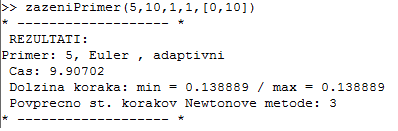
\includegraphics[scale=1]{a1}
			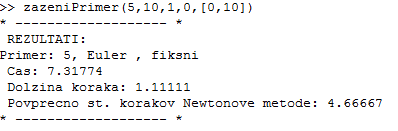
\includegraphics[scale=1]{a2}
			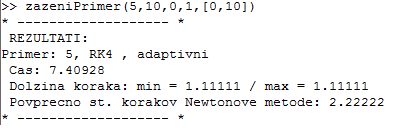
\includegraphics[scale=1]{a3}
			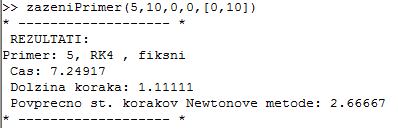
\includegraphics[scale=1]{a4}
		\end{minipage}%
	\end{figure}	
	\newpage
	Po izvajanju tega postopka za vse primere smo dobili naslednje rezultate: \\ \\
	\begin{tabular}{|c | c | c | c | c |} 
		\hline
		\textbf{Funkcija} &\multicolumn{2}{|l|}{\textbf{Euler}} &\multicolumn{2}{|l|}{\textbf{RK4}}\\                
		\small &adaptivno & fiksno & adaptivno & fiksno \\ 
		\hline
		\small{}$f_{1}(x,y,z)=x^{2} + y^{2}+ z^{2}=4$ & & & &\\ 
		\small{}$f_{2}(x,y,z)=x^{2} + y^{2}    =1$  & 3 & 5 & 3 & 3.222 \\
		\hline
		\small{}$f_{1}(x,y,z)=x^{2} + y^{2}+ z^{2}=4$ & & & &\\ 
		\small{}$f_{2}(x,y,z)$ = $3x + 2y + z = 1$  & 3 & 4.222 & 3 & 3.333 \\
		\hline
		\small{}$f_{1}(x,y,z)=x^{2} + y^{2}+ z^{2}=4$ & & & &\\ 
		\small{}$f_{2}(x,y,z)$ = $y^4 + log(x^2 + 1)z^2 - 4 = 1$  & 3 & 5 & 3 & 3.222 \\
		\hline
		\small{}$f_{1}(x,y,z)$ = $x^2 + cos(y)z^2 - 12 = 4$ & & & &\\ 
		\small{}$f_{2}(x,y,z)$ = $y^4 + log(x^2 + 1)z^2 - 4 = 1$  & 3 & 4.111 & 2.222 & 2.556 \\
		\hline
		\small{}$f_{1}(x,y,z)$ = $e^{(-x^{2}+1)}+y^{2}+z^{2} = 3$ & & & &\\ 
		\small{}$f_{2}(x,y,z)$ = $e^{(xyz)}+y^{2}+z^{2} = 10$  & 3 & 4.667 & 2.222 & 2.667 \\
		\hline
		\small{}$f_{1}(x,y,z)$ = $e^{(-x^{2}+1)}+y^{2}+z^{2} = 3$ & & & &\\ 
		\small{}$f_{2}(x,y,z)=x^{2} + y^{2}+ z^{2}=4$  & 3 & 5 & 3 & 3.222 \\
		\hline
		\small{}$f_{1}(x,y,z)$ = $e^{(-x^{2}+1)}+y^{2}+z^{2} = 3$ & & & &\\ 
		\small{}$f_{2}(x,y,z)=x^{2} + y^{2}    =1$  & 3 & 5 & 3 & 3.333 \\
		\hline
		\small{}$f_{1}(x,y,z)$ = $e^{(xyz)}+y^{2}+z^{2} = 10$ & & & &\\ 
		\small{}$f_{2}(x,y,z)=x^{2} + y^{2}    =1$  & 3 & 5 & 3 & 3.556 \\
		\hline
	\end{tabular}
	\newline
	\newline
	Pri bolj kompleksnih funkcijah kot so npr.:
	\begin{itemize}
		\item $f_{1}(x,y,z)$ = $x^2 + cos(y)z^2 - 12 = 4$  in \item $f_{2}(x,y,z)$ = $y^4 + log(x^2 + 1)z^2 - 4 = 1$,
	\end{itemize}
	smo dobili pri adaptivnem koraku manjše povprečno število korakov, ker je metoda hitro konvergirala, vendar za to ceno zmanjšala korak in delovala počasneje (približek je bil blizu pravilne rešitve, saj je bil premik majhen). Tudi minimalno in maksimalno število korakov sta bila manjša kot pri vseh ostalih. Adaptivni korak se pri teh funkcijah približa spodnji meji (2), dolžina koraka pa se manjša. 
	\par Pri fiksnem koraku smo prišli do podobnega zaključka kot pri adaptivnem, da bolj kompleksne funkcije hitreje konvergirajo, saj mora biti korak manjši (ni prikazano v tabeli).
	
	\newpage
	\section{Koda}
	\begin{lstlisting}[language=Octave]
	
	\end{lstlisting}
	\newpage
	\section{Delitev dela v skupini}
	\subsection{Programerski del}
	\begin{itemize}
		\item Aljaž: Adaptivni korak, test skripta
		\item Lina: Reševanje primerov, empirično določanje parametrov
		\item Blažka: Ogrodje programa, združitev funkcij, test skripta
		\item Luka: Reševanje primerov, empirično določanje parametrov
	\end{itemize}
	\subsection{Poročilo}
	\begin{itemize}
		\item Aljaž: Adaptivni korak, Jacobijeva matrika
		\item Lina: Analiza, primeri, testiranje
		\item Blažka: Predstavitev problema, opis modela in metod
		\item Luka: Opis modela in metod (primeri delovanja)
	\end{itemize}
	\section{Reference}
	\begin{itemize}
		\item Zapiski s predavanj: Diferencialne enačbe
		\item \url{https://en.wikipedia.org/wiki/Euler_method}
	\end{itemize}
\end{document}
